\documentclass{article}
\usepackage[utf8]{inputenc}
\usepackage{tikz}
\usetikzlibrary{positioning}
\usetikzlibrary{shapes}

\begin{document}

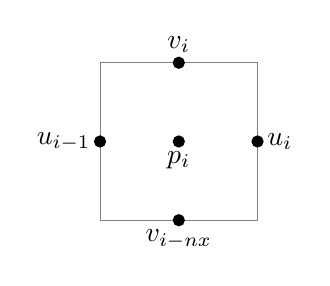
\begin{tikzpicture}
%grid
%horizontal
\draw[gray, thin] (0,0) -- (2,0);
\draw[gray, thin] (0,2) -- (2,2);
%vertical
\draw[gray, thin] (0,0) -- (0,2);
\draw[gray, thin] (2,0) -- (2,2);
%nodes
\filldraw [black] (2,1) circle (2pt) node[anchor=west]{$u_i$};%ui
\filldraw [black] (0,1) circle (2pt) node[anchor=east]{$u_{i-1}$};%ui-1
\filldraw [black] (1,2) circle (2pt) node[anchor=south]{$v_i$};%vi
\filldraw [black] (1,0) circle (2pt) node[anchor=north]{$v_{i-nx}$};%vi-1
\filldraw [black] (1,1) circle (2pt) node[anchor=north]{$p_i$};%pi

\end{tikzpicture}
\end{document}